\section{Design goals: a high level of co-presence}

In this section, we explore the design goal of our system: a high level of co-presence. Co-presence in tele-communication is defined as that distributed users feel like at the same location at the same time \cite{kraut2002use}. Thus, we analyze the requirements of co-presence in two aspects: temporal synchronicity and spatial synchronicity.

\subsection{Temporal Synchronicity}

Temporal synchronicity means that multiple users communicate and interact with each other at the same time. We identify two requirements for temporal synchronicity. First, a low network delay within 50 ms. Second, an optional sync assistance to make sure that users perform at the same time if necessary.

\subsubsection{Low network delay}

We recommend a low end-to-end delay of 50 ms in 3D telepresence, i.e, the time interval between a user acts and his partner sees.

As we reviewed, an one-way delay of 100 ms to 150 ms can support most applications in audiovisual communication. Most tasks in prior work are based on turn taking, e.g., face-to-face conversation, teleconference and so on. Users might confuse network delay with others' response time, which yield to a less sensitiveness of network delay. In a 3D telepresence system with co-presence, the communication may involve more synchronous tasks. For example, users doing handshake may be more sensitive to the network delay.

There are some tasks that indeed need a very low network delay. For examples, a musical collaboration needs an one-way delay of 30 ms to 50 ms \cite{schuett2002effects}, the Rock-Paper-Scissors game requires 40 ms to 70 ms \cite{hashimoto2006influences}.

The analysis of end-to-end delay is ignored by most existing 3D telepresence systems \cite{maimone2011encumbrance, kurillo2008immersive, petit2010multicamera, pejsa2016room2room}. Some systems provide data of frame rate and network latency of frames so that we can assess their end-to-end delay. However, most of them are far away from the requirement of high temporal synchronicity \cite{gross2003blue, beck2013immersive, gibbs1999teleport}. Holoportation \cite{orts2016holoportation} is quite responsive, but there is still a gap of about 30 ms between its performance and our design goal.

\subsubsection{Sync assistance}

We recommend an optional sync assistance design to make sure that the users can perform at the very same time. Though the network delay is unavoidable in the audiovisual transmission, it is possible to accurately synchronize the timing of two systems through the Network Time Protocol (NTP) \cite{mills1991internet}. We can therefore give simultaneous audio or visual cues for both users to help their synchronization of task.

We have two reasons for this design goal. First, it is necessary to make sure that two users perform at the same time in some tasks. For examples, simultaneity is the key to fairness in the Rock-Paper-Scissors game and the quality in a musical collaboration.

Second, as \cite{hashimoto2006influences} revealed, the caller who try to synchronize the actions may well experience the round-trip delay while his partner perceive no delay because he just adjusts the timing of his motion to the caller' s timing. However, with the help of sync assistance, the round-trip delay will be halved into two one-way delay.

\subsection{Spatial Synchronicity}

Spatial synchronicity means that multiple users feel like at locating at the same place. We identify two requirements of spatial synchronicity. First, multiple users share the same space. Second, multiple users share the same objects.

\subsubsection{Shared space}

There are two benefits that distributed users can share a space. First, to share the same location, e.g., the users can visually touch each other, change their relative locations and so on. Second, the users can share the same sense of direction. The problems of pointing and eye contact in 2D are easily solved by the shared 3D space.

As we stated above, HMDs and SIDs are the most practical ways to support high immersion of 3D. We recommend HMDs because it naturally support the shared location and direction. The rendering of HMD occurs exactly in front of users' eyes. On the contrary, users in SIDs wear 3D glasses to match the binocular images rendered on surround-screen projection. There are two drawbacks of the SID rendering. First, users themselves and surrounding physical objects may hinder their sight. Second, SID cannot render virtual objects in a very short distance, otherwise it would cause visual discomfort. The interaction in SID systems always occurs through a 'window' screen between one space and the other. \cite{orts2016holoportation}. Thus, a simple handshake action is not supported by SID.

To the best of our knowledge, the most practical way to allow shared space is to render live 3D reconstruction in HMDs. Currently, this design is only supported by a small portion of 3DTI systems \cite{orts2016holoportation, maimone2013general, lindlbauer2018remixed, smith2018communication}.

\subsubsection{Shared props}

A shared prop is an virtual object that is merged by two similar physical objects in the two ends. Imaging a remote chess game in 3D telepresence, two users can  interact physically with a chessboard and the chess pieces on his own side. A future 3D telepresence system is able to fuse two physical chessboards into one, while retaining all the chess pieces in both ends. So the user has his own chess pieces, and can see his partner' s chess pieces virtually.

The design of supporting shared props has two advantages. First, it provides tactile feedback of shared props for both  users. Second, physical objects provide common ground for the communication, and a successful communication relies on a foundation of mutual knowledge or common ground \cite{clark1981definite, clark1990referring}.

Shared props have not yet been supported by prior work. In TeleCP, we set up a design goal that supports distributed users to share same objects by merging similar physical objects in both ends.

%In this section, we explore the design goals of our system. We want our system to support more killer applications of 3DTI. To do this, we first performed a brainstorming about the possible applications in 3DTI. Then, we summarize the necessary requirements to support the proposed applications as our design goals. They are: \emph{rich visual information}, \emph{spatial co-presence}, \emph{high synchronicity} and \emph{shared props}. These design goals are in fact different extents of co-presence that two users feel like at the same location at the same time \cite{kraut2002use}. Thus, the design goals of our system can be summed up to a high level of co-presence. 

\subsection{Possible applications of TeleCP}

%The goal of the brainstorming was to collect killer applications in 3DTI that are either impossible or unnatural in prior tele-communications. Finally, we obtained nine typical application.

In summary, the design goals of TeleCP is to support a high level of co-presence. It consists of two parts: temporal synchronicity (low network delay, sync assistance) and spatial synchronicity (shared space, shared props). Among these goals, shared space is naturally supported by 3D reconstruction and HMD rendering, while other goals will be supported by our software framework.

We give examples of possible applications with these design goals and analyze the detailed requirements of these applications.

\begin{itemize}
    \item (1) \emph{Handshake}: A handshake can convey information of a person’s personality \cite{chaplin2000handshaking} and express the friendship \cite{bardeen1970interpersonal}. TeleCP allows two users to visually touch with each other, so that the distributed users can shake their hands.

    \item (2) \emph{Musical collaboration}: Development of audio transport over network have been able to support professional-level musical collaboration \cite{carot2007networked, carot2007network}. However, the audio channel is not sufficient enough for a successful performance. 3D telepresense can support a vivid musical collaboration. Notice that musical collaboration requires a low one-way network delay of 30 ms to 50 ms \cite{schuett2002effects}.
    
    \item (3) \emph{Piano duet}: Piano duet is a special form of musical collaboration that involves two players performing at one instrument. TeleCP has the potential to fuse two physical pianos into a shared piano in the virtual space. The virtual piano is a typical shared prop.
    
    \item (4) \emph{Dance collaboration}: Dance is a collaborative art form that involves multiple dancers in one space. During a dance, dancers may change their relative locations. In a networked situation, dance collaboration is only supported by a 3D telepresence system with spatial synchronicity.
    
    \item (5) \emph{The Rock-Paper-Scissors game}: The game is a face-to-face interaction in a short distance, which may be more natural in the 3D environment. It requires the players to show a gesture at the same time. As \cite{hashimoto2006influences} suggests, a one-way delay of 50 ms is needed for the networked Rock-Paper-Scissors game.
    
    \item (6) \emph{Teleconference}: Teleconference is a typical conversation task in 2D communications \cite{allen1996teleconferencing, marlow2016beyond}. 3D telepresence offers richer visual information for the teleconference. For example, a user can observe the partner's body language to better understand the conversation.
    
    \item (7) \emph{Building blocks}: Building blocks is a tele-collaboration task that two users collaborate to build 3D blocks in a given configuration \cite{orts2016holoportation}. Each user has only part of the objects and can see the blocks of his partner virtually.
    
    \item (8) \emph{The chess game}: The chess game involves two players at one chessboard. It is possible for a 3D telepresence system to support a remote chess game. In physical world, each player interacts with a chessboard and the chess pieces on his own side. The system fuses the two chessboards into one and shows the chess pieces in both ends at the same time.
\end{itemize}{}

\begin{table}[!htbp]
\begin{tabular}{|l|l|l|l|l|l|l|l|l|}
\hline
\textbf{Design goals} & 1       & 2           & 3           & 4           & 5           & 6           & 7           & 8       \\ \hline
low network delay                      & $\surd$ & $\surd$     & $\surd$     & $\surd$     & $\surd$     & $\triangle$ & $\triangle$ &         \\ \hline
sync assistance                        &         & $\triangle$ & $\triangle$ & $\triangle$ & $\triangle$ &             &             &         \\ \hline
shared space                           & $\surd$ & $\triangle$ & $\surd$     & $\surd$     & $\triangle$ & $\triangle$ & $\surd$     & $\surd$ \\ \hline
shared props                           &         &             & $\surd$     &             &             & $\triangle$ & $\triangle$ & $\surd$ \\ \hline
\end{tabular}
\caption{The requirements of each proposed application. "$\surd$" means that the design goal is necessary. "$\triangle$" means that the design goal can improve the interaction.}
\label{tab:brainstorming}
\end{table}

As table \ref{tab:brainstorming} shows, a 3D telepresence system can support more applications or improve the interaction in a more natural manner if it supports the four design goals we proposed. In the next section, we will discuss the implementation of our system to support these goals.
















%Rich visual information is an apparent advantage of 3DTI that benefits from the 3D vision. It has two aspects. The first is motion parallax, i.e., the user can change his point of view and direction of gaze naturally in a 3D environment \cite{fuchs2014immersive}. The second is binocular vision, e.g., the combined field of view is larger, depth perception is much better and so on \cite{kooi2004visual}.

%The ability that a 3DTI system can support visual information depends on its rendering approach. Both HMDs and SIDs support a rich visual information. Some 3DTI systems use a simplified form of SID called head-tracked auto-stereo display \cite{maimone2011encumbrance, maimone2012real, pejsa2016room2room}. They only support motion parallax but not binocular vision. Some user studies on 3DTI were conducted with 2D displays \cite{wu2009quality, wu2010m}, which indicates the lack of related technical supports for HCI research.

% [abandon] below
\iffalse

\subsubsection{High synchronicity}

Co-presence is that distributed users feel like locating at the same place at the same time \cite{kraut2003visual}. The temporal part of co-presence, high synchronicity, is usually forgotten by researchers. For audio-mediated communications, one-way delay of 150 ms has been a standard that provides a good user experience \cite{recommendation2003114}. For visual telecommunication systems, \cite{tam2012video} suggests a network delay under 200 ms is not noticeable for most users.

We recommend a low end-to-end delay of 50 ms in 3DTI, i.e, the time interval between a user acts and his partner sees. As table \ref{tab:brainstorming} shows, many possible applications in 3DTI require for high synchronicity. For examples, a musical collaboration needs an one-way delay of 30 ms to 50 ms \cite{schuett2002effects}, the Rock-Paper-Scissors game requires 40 ms to 70 ms \cite{hashimoto2006influences}. The difference between 2D and 3D can be explained. Most tasks in 2D are based on turn taking (e.g., teleconference and video chat) because of the lack of co-presence. In contrast, 3DTI applications might involve synchronous actions or sounds that can easily reveal the network delay.

The analysis of end-to-end delay is ignored by most existing 3DTI systems \cite{maimone2011encumbrance, kurillo2008immersive, petit2010multicamera, pejsa2016room2room}. Some systems provide data of frame rate and network latency of frames so that we can assess their end-to-end delay. However, most of them are far away from the requirement of high synchronicity \cite{gross2003blue, beck2013immersive, gibbs1999teleport}. Holoportation \cite{orts2016holoportation} is quite responsive, but there is still a gap of about 30 ms between its performance and our design goal.



% [paragraph] The structure of this subsection.
In this section, we first explore how users perceive network delay in tele-communications based on a systematic review and analysis of prior works. We introduce three cues of delay perception: \emph{synchronous cues}, \emph{conversation} and \emph{visual feedback}, in the order from strong to weak. Next, we summarize the characters of 3D communications. We suggest that more tasks in 3D involve \emph{synchronous cues}, which require a low network delay. Last, we draw a hypothesis: users are less sensitive and more tolerable to network delay in conversations in 3D.

% through a systematic review and analysis of prior works

\subsection{How users perceive network delay?}

Users perceive network delay by cues. The cues can be divided into two categories: synchronous cues and turn-based cues. A synchronous cue is that the two users speak or gesture at the very same time. It is the strongest cue to reveal network delay. A user perceives the delay once he feel that the partner acts slower than himself. Thus, we define the most delay-sensitive level as (L1) \emph{synchronous tasks}, which involves synchronous cues in the interaction.

A turn-based cue is that the users take turn speaking or gesturing. The turn gap is defined as the time between a user finishes a turn and his partner responses. It is uncertain but somehow predictable. In a networked communication, the network delay prolongs the perceived turn gap. As figure xxx shows, the perceived turn gap is the sum of actual turn gap and the round-trip delay.

[图] maybe there should be a figure to illustrate that: perceived turn gap = actual turn gap + round-trip delay. The easier to predict the actual turn gap is, the easier the network delay can be perceived. 

The turn gap is uncertain but somehow predictable. When the network delay is low, the user can not judge if the prolonged turn gap is caused by the network delay or by the slow response of his partner. When the network delay becomes higher, the user feels that the turn gap is abnormal, hence he notice the network delay. Because of the uncertain turn gap, turn-based cues are the weaker cues for delay perception compared to synchronous cues.

Turn-based cues contain conversation (with audio channel) and visual feedback (without audio channel). Previous theories [?] suggests that the turn gap of a conversation is generally easier to predict compared to the visual feedback. The more predictable the turn gap is, the easier the user perceives the network delay. Correspondingly, related studies in 2D reveals that conversation make users sensitive to the network delay in a turn-based task [?]. Thus, we define the second delay-sensitive level of tasks as (L2) \emph{turn-based audiovisual tasks}. We regard (L3) \emph{turn-based visual-only tasks} as the less delay-sensitive one.

Next, we introduce the theoretical background to further explain the problem. We refer local delay perception to \emph{synchronous tasks}, Turn-Taking Model and Grounding Theory to \emph{turn-based audiovisual tasks}, and Situation Awareness Theory to \emph{turn-based visual-only tasks}.

\subsubsection{Local delay perception}

For local delay, 100 ms is an upper boundary for users to fell that the system is running instantaneously \cite{nielsen1993response}. For a better performance, a local delay of 30 ms to 50 ms is needed \cite{chen2007review}. In a \emph{synchronous task}, the users are expected to act exactly at the same time. The users can perceive the network delay if their actions are obviously out of sync. We deem that users' ability to perceive the delay in this situation is similar to the perception of a local delay.

\subsubsection{Bad case: the round-trip delay}

Many \emph{synchronous tasks} require one of the users to synchronize the actions by gesturing or saying something, e.g., "Three, two, one, go!". As \cite{hashimoto2006influences} revealed, there is a difference between the delay perceptions of the \emph{caller} and the other user \emph{replier}. The \emph{caller} is the user who try to synchronize the actions. As figure \ref{fig:caller_and_replier} shown, the \emph{caller} starts a Rock-Paper-Scissors game. The \emph{replier} just adjusts the timing of his motion to the \emph{caller's} timing. Thus, he do not perceive any network delay. In contrast, the \emph{caller} experiences the round-trip delay before seeing the partner's reaction. The round-trip delay may destroy the user experience in \emph{synchronous tasks}. We should balance the perceived network delay of the the two users.

\begin{figure}[!htbp]
\centering
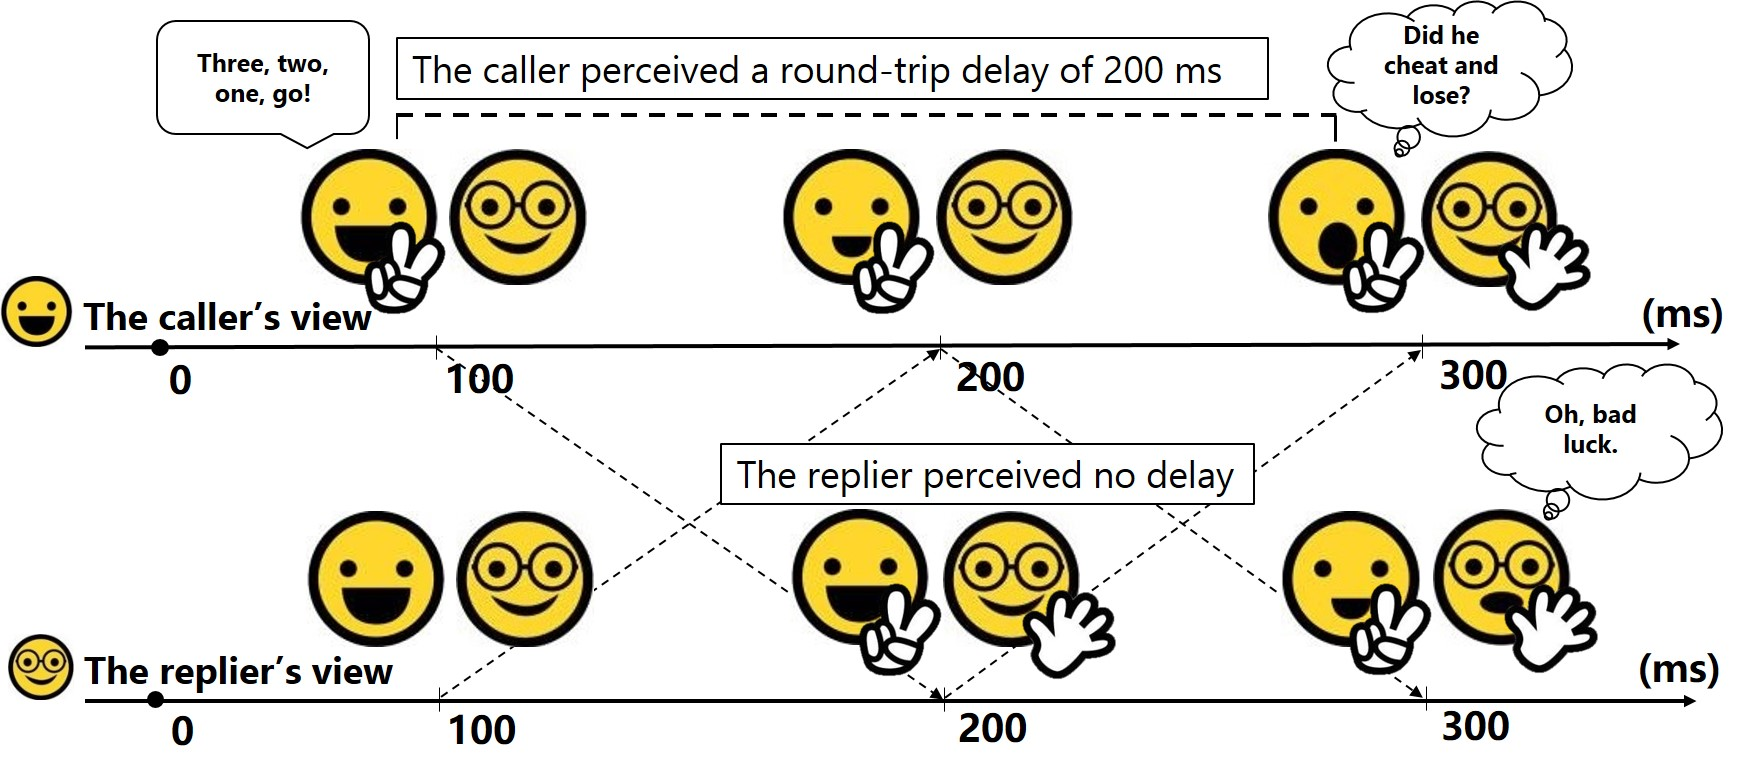
\includegraphics[width=1.0\linewidth]{figures/figure_caller_and_replier.jpg}
\caption{In a networked \emph{Rock-Paper-Scissors} game with a delay of 100 ms, the \emph{caller} is the player who try to synchronize the game, e.g., by saying "Three, two, one, go". He perceives a round-trip delay of 200 ms, while his partner perceives no delay.}
\label{fig:caller_and_replier}
\end{figure}

\subsubsection{Turn-Taking Model}

Turn taking is a part of universal infrastructure for language \cite{levinson2016turn}. In daily life we have learned to unconsciously manage a conversation by using the timing of the small pauses in speech \cite{sacks1978simplest}. Figure \ref{fig:turn_taking} shows the typical timing of the conversation. A Turn is 2 s in average. The language production system is slow: preparation before output begins takes 600 ms to 1500 ms \cite{indefrey2004spatial, bates2003timed, griffin2000eyes}. However, switching of speakers is rapid, because the turn taking system relies on prediction \cite{levinson2016turn}. The modal turn gap is around 200 ms \cite{levinson2015timing}.

\begin{figure}[!htbp]
\centering
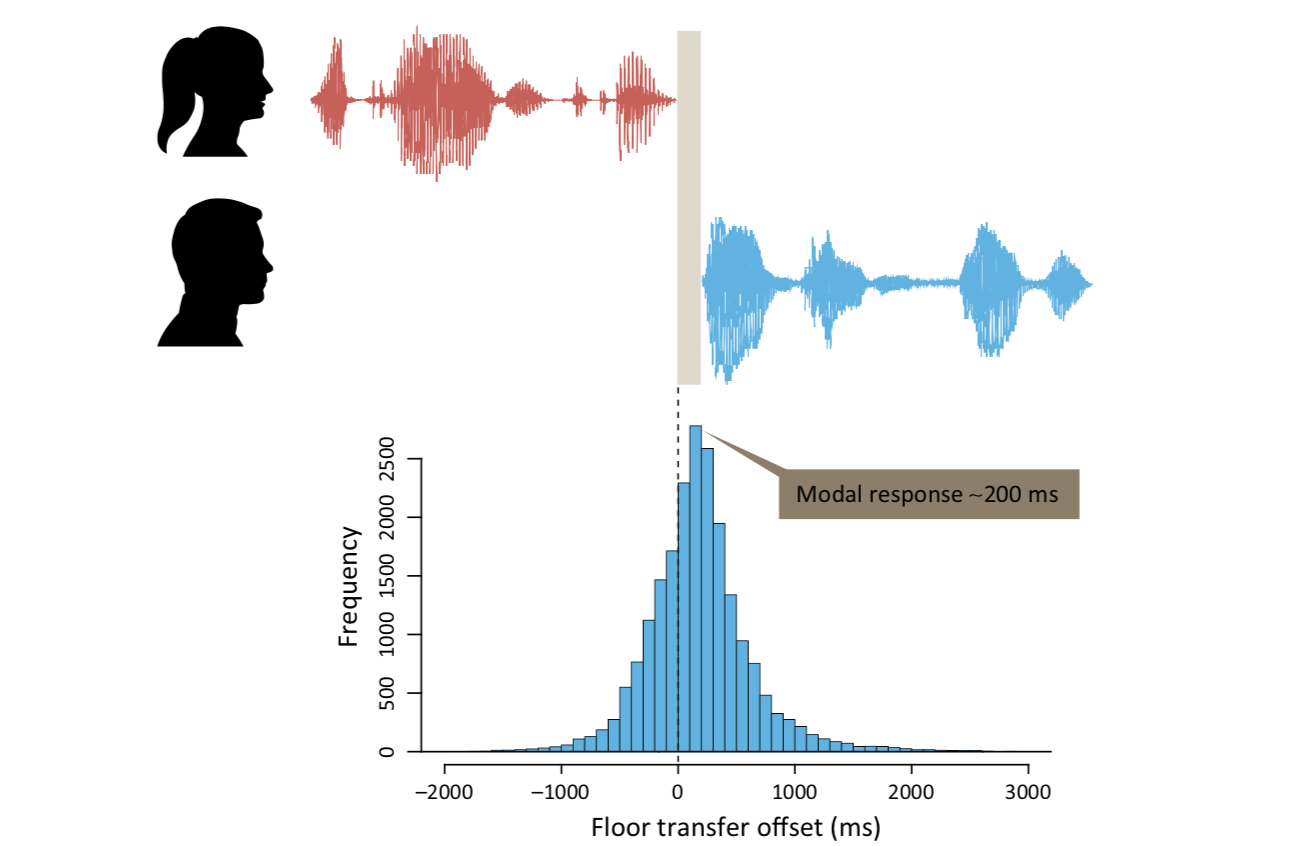
\includegraphics[width=1.0\linewidth]{figures/figure_turn_taking.png}
\caption{[注意,这是盗图] Turn Taking Model.}
\label{fig:turn_taking}
\end{figure}

As Turn-Taking Model suggests, the turn gap of a conversation is short and predictable because of our daily life training. As we explain above, the more predictable the turn gap is, the easier the user perceives the delay. Thus, conversation is also an important cue for delay perception. Previous studies have found that the users are sensitive to network delay in a conversation. Delay of 100 ms is noticeable in audio communications \cite{wang2010evaluation, itu2003recommendation, recommendation2003114}. Delay of 150 ms becomes industrial standard of the telephone network \cite{recommendation2003114}. Delays greater than 450 ms can severely impact communication \cite{gergle2006impact, o1997characterizing, tang1992users}.

\subsubsection{Situation Awareness Theory}

Situation Awareness Theory holds that visual information helps pairs assess the current state of the task and plan future actions \cite{endsley2017toward, endsley2000situation}. A user need to maintain an on-going awareness of the partner' s actions and the status of the task objects. Through the observation of the turn gap, a user may perceive the network delay. However, the turn gap of an visual feedback is hard to predict [?]. Thus, users are less sensitive to the network delay in a \emph{turn-based visual-only task}. Previous works shows that the network delay requirement of the 2D \emph{turn-based visual-only tasks} is from xxx ms to xxx ms [?, ?, ?].

\subsubsection{Grounding Theory}

Grounding Theory suggests that a successful communication relies on a foundation of mutual knowledge or common ground \cite{clark1981definite, clark1990referring}. Visual information is an important source of common ground that provides evidence of comprehension for communication \cite{brennan2005conversation, kraut2003visual}. Sufficient visual information can assist the verbal communication \cite{gergle2006impact} and reduce users' dependence on conversation. For example, a user can point at an object in the shared virtual space and refer to it using a simple pronoun "that". Because visual information reduces the dependence of conversation, we suggest that users is less sensitive to delay in 3D.

\vspace{0.2cm}

In conclusion, \emph{synchronous tasks} require for the lowest network delay. The delay requirement of \emph{turn-based tasks} are looser. Among \emph{turn-based tasks}, the tasks with audio channel (conversation) require a lower network delay.

\subsection{What is new in 3D?}

There are two new features in 3D: the support of co-present and the enriched visual information. An advanced 3DTI system reconstructs the physical scene and render it in full 3D. It allows co-present, that is, the two users feel like exactly in the same virtual space. Meanwhile, 3DTI offer more visual information compared to the 2D systems, e.g., the user can perceive the distance to an object and observe it from different view points.

\subsubsection{Co-present}

Co-present is a critical feature in a full 3D tele-immersion system \cite{orts2016holoportation, whittaker2003things, kraut2003visual}. In previous 2D communications and even the 3DTI systems without HMDs, the interaction always occurs through a ‘window’ from one space into the other. Co-present allows the users to "touch" each other, to exchange their locations freely, to use the shared physical props \cite{luff1998mobility} and so on. The significance of co-present is that 3DTI supports many impossible tasks in 2D or improve some existing tasks in a more natural manner. For example, as the users can "touch" each other in 3DTI, human can finally shake hands in distributed places.

\subsubsection{Rich visual information}

3DTI renders the virtual space in 3D. A 3D environment offer richer visual information compared to the 2D situation. First, when the user move in the virtual space, his view dynamically changes according to his location. Second, the binocular visualization allows users to perceive distance in the virtual space. The significance of the rich visual information is twofold: first, it enables 3DTI to support more tasks; second, it further reduces users' dependence on conversation, which may lead to the less sensitiveness of network delay.

\vspace{0.2cm}

We give examples for each level of tasks. They show the possibility of 3DTI. Among the examples below, the tasks with the marker '*' is only supported by 3DTI:

\begin{itemize}
    \item \emph{Musical collaboration (L1)}: Development of audio transport over networked have supported professional-quality musical collaboration \cite{carot2007networked, carot2007network}. The emerging 3DTI may support a vivid musical collaboration in the future.
    \item \emph{Piano duet (L1)*}: It is possible for a 3DTI system to fuse similar objects in both sides. Imaging there are two same pianos in two distributed rooms. 3DTI can fuse the two pianos into a virtual one, so that two distributed musicians can play piano duet.
    \item \emph{Dancing together (L1)*}: In the virtual space of 3DTI, two users can exchanges their locations freely. It allows them to dance together.
    \item \emph{Shaking hands (L1)*}: 3DTI allows the two users to "touch" with each other, so that they can shake hands.
    \item \emph{The Rock-Paper-Scissors game (L1)}: The game requires the players to show a gesture at the same time. In physical world, a pair usually play in a very short distance. We deem that it is more natural in 3D communications.
    \item \emph{Teleconference (L2)}: Teleconference is a typical tasks in 2D communications. It is a good example for remote conversation. 3DTI offers more visual information for the teleconference.
    \item \emph{Building blocks (L2)}: It is a tele-collaboration task that a user imitates the other to build blocks. Though it is possible in 2D, it will be easier in 3D because the imitator can observe the remote blocks from different view points.
    \item \emph{Remote interview (L2}: In an interview, it is important to preserve a dignified deportment. 3DTI offers more visual information about the interviewees.
    \item \emph{Playing chess (L3)*}: Each player interacted with a chessboard and chess pieces on his own side. 3DTI fuses the two scenes into a virtual one, so that each player could see both sides of chess pieces.
    \item \emph{Surgery simulation (L3)*}: The surgery simulation is between a nurse and a surgeon. For example, the nurse can prepare tools and materials in advanced by observing the actions of the surgeon.
\end{itemize}{}

\subsection{More tasks fall into the most delay-sensitive level \emph{synchronous tasks}}

3DTI supports co-present and provides more visual information. As the examples shown above, 3DTI is possible to support more tasks or improve them in a more natural manner. The new supported tasks is mostly belongs to L1 and L3. The reason for the increasing L1 is that most of these tasks require for co-present. The increment of L3 is because visual information is usually not sufficient in 2D communication.

In particular, we have to pay attention to the increasing L1 (\emph{synchronous tasks}) in 3D, because their network delay requirement is very challenging. Table xxx shows some previous studies on delay perception of \emph{synchronous tasks}. We suggest that a network delay of about 50 ms is required.

--------------------

\emph{Musical collaboration} \cite{schuett2002effects} 30 ms $\sim$ 50 ms

\emph{The Rock-Paper-Scissors game} \cite{hashimoto2006influences} 40 ms $\sim$ 70 ms

--------------------

[表格 xxx] The recommend network delay is the threshold that can provide a good experience. We summarize it according to the standard of 3.5 Mean Opinion Score (MOS) \cite{enderes2002impact, schaefer2002subjective} or the description of the paper.

\subsection{The less sensitiveness and more tolerance to network delay in 3D conversation}

In 2D, video weaken the negative impact of delay in remote interactions, because audiovisual interaction allows users to see visual information \cite{tam2012video}. As table xxx shown, there is a obvious tendency that tasks rely more on the audio channel require for a lower network delay.

--------------------

\emph{turn taking} \cite{kitawaki1991sub} 150 ms

\emph{The Rock-Paper-Scissors game} \cite{hashimoto2006influences} 40 ms $\sim$ 70 ms

\emph{3D Visual Communication} \cite{wu2009quality} 120 ms [??? bad case]

\emph{Video Group Discussion} \cite{schmitt2014asymmetric}  500 ms

\emph{Audiovisual telecommunication} \cite{tam2012video} 500 ms

--------------------

[表格 xxx] The recommend network delay is the threshold that can provide a good experience. 在总结论文的时候,作者人工给这些tasks定性:纯语音、偏语音、语音视频都重要、偏视频或是纯视频。

We deem that this effect enhances in 3D. According to Turn-Taking Model [?] and Grounding Theory, the users are more sensitive to the delay of conversation compared to visual feedback. Visual information reduce users' dependence on audio communication, so the sensitiveness of delay is decreased accordingly. As \cite{kraut2002use, kraut2003visual} suggests, when all parties to the interaction are co-present, the users share a rich visual space. Thus, 3DTI systems with co-presence provide the richest visual information. We suggest that the users are less sensitive and more tolerable to the network delay in 3D.

We suggest that in 3D, the network delay requirement is 250 ms for (L2) \emph{turn-based audiovisual tasks} and 300 ms for (L3) \emph{turn-based visual-only tasks}.

\subsection{Suggestions for network design}

% [paragraph] We present the framework. The three level, its delay.
The framework classify 3DTI tasks by their requirement of network delay. There are three levels:

\begin{itemize}
    \item \textbf{(L1) \emph{synchronous tasks}}: The tasks with synchronous voices or actions, e.g., shaking hands, dancing together and musical collaboration.
    \item \textbf{(L2) \emph{turn-based audiovisual tasks}}: The tasks with conversation and turn-based actions, e.g., teleconference and remote interview. The audio channel is available.
    \item \textbf{(L3) \emph{turn-based visual-only tasks}}: The tasks with turn-based actions, e.g., playing chess and surgery simulation. The audio channel is not available.
\end{itemize}

% introduction: we give this suggestion according to the new feature of network service and network experience in 3D.
There is a space to improve the network design for a 3DTI system. Both the system service and the user experience in 3D are different from the 2D situation. On the one hand, the computation is tough in 3D, which leads to a generally longer computing time. The bandwidth requirement is also larger (1.5-fold of a 1080p video [?]); On the other hand, users' perception of network delay change a lot in 3D. The practitioners can suit their methods to the situation when designing the networked applications:

\subsubsection{Zero-delay audio assistance (for L1)}
    
In \emph{synchronous tasks}, the users are sensitive to the network delay. Moreover, as we explained above, the \emph{caller} may perceive a round-trip network delay. To improve the user experience, we suggest to add a zero-delay audio prompt tone in the application. In the networked \emph{Rock-Paper-Scissors} game, for example, we can add synchronized sounds of "tick, tick, tack" for both the users. The users can show their gesture when they hear the "tack" sound so that the actions can be exactly at the same time. The advantage of this strategy is twofold: first, to avoid the round-trip network delay; second, the psychological hint of fair game.
    
Though the network delay is unavoidable in the audiovisual transmission, it is possible to accurately synchronize the timing of two systems through the Network Time Protocol (NTP) \cite{mills1991internet}. Thus, this strategy is practicable. In our experiment, we validated that this strategy can significantly improve the user experience.
    
\subsubsection{Trade bandwidth for time (for L1)}
    
In general, delay and bandwidth are a trade-off in network transmission. Compression is the key. It reduce the bandwidth requirement of a 3DTI network. Recent works on 3D data compression shows that a bandwidth of tens of megabits per second is possible to support a 3DTI system \cite{collet2015high, de2016compression}. However, compression is time-consuming. Some compression methods are based on inter prediction, which leads to several frames of latency.
    
The \emph{synchronous tasks} require a network with delay of 50 ms. The service has almost no time for compression. In this situation, we can trade bandwidth for time, i.e., to use a lightweight compression method, or even transmit the raw data directly (about 500 Mbps). This strategy can reduce the network delay as well as maintain the highest quality. The price of this strategy is the very high requirement of network bandwidth. Thus, it is only possible if the practitioners have a dedicated network.
    
\subsubsection{Buffer frames to recover lost packets and deal with jitter (for L2 and L3)}
    
Delay is not the only factor that affects the user experience in a networked communication. Jitters, delay spikes and network losses will degrade the user experience as well. Fortunately, the network requirement of turn-based tasks are looser in 3D. Compared to the 2D situation, we have extra 50 ms $\sim$ 100 ms for recovering lost packets and smoothing data stream .

\subsubsection{Trade time for bandwidth (for L2 and L3)}
    
As we explained above, delay and bandwidth are a trade-off. For turn-based tasks, we can trade time for bandwidth, i.e., to use a heavyweight compression method. The state-of-the-art 3D reconstruction pipelines \cite{orts2016holoportation, dou2016fusion4d} track live 3D model based on temporal consistency. It provide convenience for the compression of data stream, i.e., we can leverage inter prediction in the transmission.
    
\subsubsection{The audio can be earlier (for L2)}
    
In a \emph{turn-based audiovisual task}, the transmission of audio is more lightweight than that of the video. Coincidentally, small delay can seriously disrupt the audio communication \cite{krauss1967effects}, while the delay requirement of the video is looser. However, most video conference systems synchronize video and audio by delaying audio, which reduces the responsiveness of the conversation [?, ?, ?, ?]. \cite{isaacs1994video} suggests that we can transmit the audio a little bit faster than the video. Even if the gap between audio and video is noticeable, this strategy can somehow improve the user experience. In the 3D situation, we suggest a gap between audio and video within 100 ms is acceptable.

\fi
